\ifspanish

\question[20] % VGV

Se dispone de un sistema de comunicaciones en el que el transmisor envía, con la misma probablidad a priori, un único símbolo (``$+1$'' ó ``$-1$'') de manera simultánea por dos canales ruidosos, tal y como se ilustra en la figura:
\begin{center}
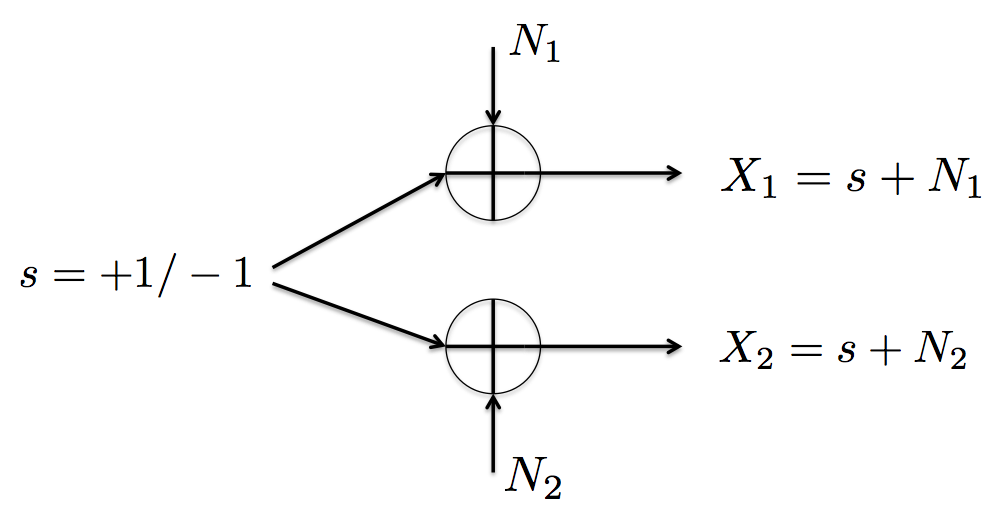
\includegraphics[width=8cm]{Figuras/Fig_canal_gauss}
\end{center}

donde $N_1$ y $N_2$ son dos variables de ruido gaussiano, independientes entre si, con medias nulas y varianzas $\lambda v$ y $(1- \lambda) v$, respectivamente, y $v>0$ y $0 \leq \lambda \leq 1$ son constantes conocidas.
\begin{parts}
\part Obtenga el decisor de mínima probabilidad de error, basado en la observación conjunta de $X_1$ y $X_2$, que permite al receptor saber si se transmitió el símbolo ``$+1$'' ó ``$-1$''.
\part Obtenga la probabilidad de error del decisor anterior.  Exprese su resultado utilizando la función:
$$F(x) = 1- Q(x) = \int_{-\infty}^x \frac{1}{\sqrt{2\pi}} \exp{\left( - \frac{t^2}{2}\right) } \; dt$$

\part Analice el comportamiento del decisor (frontera de decisión y probabilidad de error) para los casos: $\lambda=0$ y $\lambda=1$.
\end{parts}

\begin{solution}

\begin{parts}
\part $(1-\lambda)x_1 + \lambda x_2 \dunodcero 0$
\part $\displaystyle  P_{\rm e}=F(-\frac{1}{\sqrt{\lambda(1-\lambda)v}})$ 
\part Si $\lambda=0$, $X_2=s$ (tiene varianza nula) y solo se usa esta observación para decidir. $P_{\rm e}=0$. Si $\lambda=1$ ocurre lo mismo pero con $X_1$.
\end{parts}
 \end{solution}

\else

\question[20] % VGV

Consider a communication system where the transmitter sends, with equal {\em a priori} probabilities, the same symbol ``$+1$'' or ``$-1$'' through two noisy channels, as illustrated in the figure:
\begin{center}
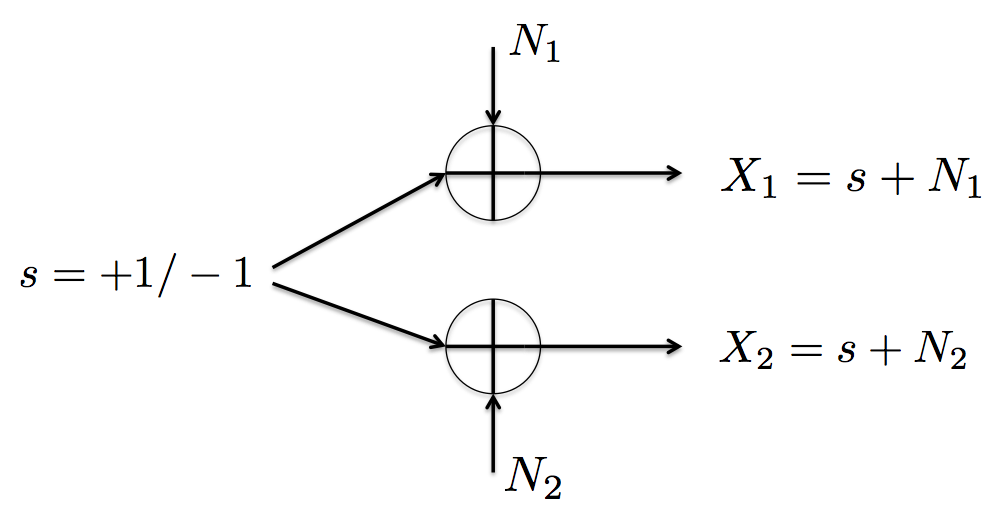
\includegraphics[width=8cm]{Figuras/Fig_canal_gauss}
\end{center}
where $N_1$ and $N_2$ are independent Gaussian random variables, with zero mean and variances $\lambda v$ and $(1-\lambda) v$, respectively; $v>0$ and $0 \leq \lambda \leq 1$ are two known constants.

\begin{parts}
\part Obtain the binary classifier with a minimum probability of error, based on the joint observation of $X_1$ and $X_2$, which allows the receiver to decide whether the transmitted symbol was $+1$ or $-1$.
\part Compute the error probability of the above decision maker. Express your result by means of the function
$$F(x) = 1- Q(x) = \int_{-\infty}^x \frac{1}{\sqrt{2\pi}} \exp{\left( - \frac{t^2}{2}\right) } \; dt$$
\part Analyze the behaviour of the decision maker (i.e., its decision rule and probability of error) when: $\lambda=0$ and $\lambda=1$.
\end{parts}

\begin{solution}
\begin{parts}
\part $(1-\lambda)x_1 + \lambda x_2 \dunodcero 0$
\part $\displaystyle  P_{\rm e}=F(-\frac{1}{\sqrt{\lambda(1-\lambda)v}})$ 
\part When $\lambda=0$, $X_2=s$ (its variance is zero) and we only consider this observation to make the decision. $P_{\rm e}=0$. When  $\lambda=1$ a similar behaviour happens, but considering observation $X_1$.
\end{parts}
\end{solution}

\fi